\chapter{PENGUJIAN DAN ANALISIS}
\label{chap:pengujiananalisis}

% Ubah bagian-bagian berikut dengan isi dari pengujian dan analisis
Pada penelitian ini dipaparkan hasil pengujian serta analisis yang dilakukan sesuai dengan desain sistem yang sudah dirancang pada bab sebelumnya. Dataset yang digunakan berasal dari \url{data.mendeley.com} ditambah dengan dataset yang berasal dari proses \textit{webcrawling} sendiri. Pengujian dilakukan dengan beberapa bagian sebagai berikut :

\begin{enumerate}[nolistsep]
    \item Pengujian Performa berdasar pada Penggalan Kata yang Diambil
    \item Pengujian Performa berdasarkan model BERT yang digunakan
    \item Pengujian Performa berdasarkan Pendekatan Cara \textit{Training}.
\end{enumerate}

Pada pengujian, masing - masing model menggunakan Google Collab dengan spesifikasi \textit{hardware} seperti yang dilampirkan pada tabel \ref{tab:specs_collab}

\begin{table}
    \caption{spesifikasi PC yang digunakan}
    \label{tab:specs_collab}
    \centering
    \begin{tabular}{|l|l|}
        \hline
        \textbf{Prosessor}            & 2 v-core Intel(R) Xeon(R) CPU @ 2.20GHz   \\ \hline
        \textbf{RAM}                  & Virtual Memory : 12GB                     \\ \hline
        \textit{\textbf{Storage}}     & SSD : 69GB                                \\ \hline
        \multirow{2}{*}{\textbf{GPU}} & Nvidia Tesla T4 16GB                      \\ \cline{2-2}
                                      & Nvidia K80 12GB                           \\ \hline
        \textbf{Sistem Operasi}       & Ubuntu 18.04.5 LTS (Bionic Beaver) 64-bit \\ \hline
    \end{tabular}
\end{table}

\section{Pengujian Performa berdasar pada Penggalan Kata yang Diambil}

Untuk saat ini, BERT hanya dapat memproses sebanyak 512 token sekaligus. Sehingga, untuk melakukan pemprosesan pada data dengan teks yang panjang, diperlukan pemotongan teks agar panjang teks menjadi sesuai.

Pengujian performa berdasar pada penggalan kata yang diambil ini bertujuan untuk mengetahui tingkat akurasi model BERT pada teks dengan cara pemotongan yang berbeda. Pembedaan ini dilakukan berdasarkan pada adanya berita yang menuliskan kesimpulan di awal, atau bisa juga menuliskan kesimpulan di akhir. Alternatif lain adalah mengambil sebagian teks di bagian awal dan mengambil sisanya di bagian akhir. Maka dari itu, dalam pengujian performa ini dilakukan dengan membagi teks pada beberapa cara memenggal kata, antara lain :

\begin{enumerate}[nolistsep]
    \item Mengambil bagian awal teks.
    \item Mengambil bagian akhir teks.
    \item Mengambil 129 token dari bagian awal teks dan 383 token dari bagian akhir teks.
\end{enumerate}

Dari total data yang berjumlah 1621 data, akan diambil 18\% nya sebagai dataset pengujian, sehingga berjumlah 292 dataset sebagai pengujian. Parameter pada pengujian untuk \textit{training} di atur agar sama untuk setiap pengujian, \textit{epoch} sebesar 7, \textit{leearning rate} sebesar 2e-5, dan \textit{epsilon} sebesar 1e-8, hal yang sama juga dilakukan pada model, pengujian ini menggunakan model BERT yang telah di-\textit{pre-trained} oleh Indobert. Untuk lebih jelasnya, silahkan lihat Tabel \ref{tab: truncate_param} yang berisi rincian parameter dan model yang digunakan untuk proses \textit{training}.

\begin{table}
    \caption{Konfigurasi Parameter Untuk Pengujian berdasarkan Pemotongan Kata}
    \label{tab: truncate_param}
    \centering
    \begin{tabular}{|l|l|}
        \hline
        \textit{\textbf{epoch}}          & 3                              \\ \hline
        \textit{\textbf{learning rates}} & 2e-5                           \\ \hline
        \textit{\textbf{epsilon}}        & 1e-4                           \\ \hline
        \textbf{model}                   & indobenchmark/indobert-base-p1 \\ \hline
    \end{tabular}
\end{table}

Keluaran dari model akan dibandingkan dengan label pada dataset, yang kemudian akan dihitung untuk menghasilkan \textit{confusion matrix}, \textit{recall, precision, accuracy} dan \textit{f1-score} sesuai dengan rumus yang telah dijelaskan pada bab tinjauan pustaka.

\subsection{Pengujian dengan Mengambil Bagian Awal Teks}

Terdapat beberapa ciri - ciri yang terdapat pada kebanyakan teks berita berbahasa Indonesia, salah satu dari ciri - ciri tersebut adalah menuliskan ringkasan berita pada paragraf awal kalimat. Format seperti ini biasanya cukup sering ditemui terutama pada berita yang memanfaatkan fitur halaman pada teks beritanya. Karenanya, pada jenis - jenis berita seperti ini, orang hanya perlu melihat beberapa kalimat awal untuk mengetahui apakah bahwa berita tersebut valid dan dapat dipercaya.

Seperti bisa dilihat pada tabel \ref{tab: const_awal}, dengan memotong teks berita pada bagian awal, didapatkan tingkat akurasi sebesar 89\% dengan nilai \textit{recall, precision, f1-score} kurang lebih sama. Selain itu, dapat dilihat juga pada kolom \textit{confusion matrix}, model yang sudah dibuat memiliki nilai FP dan FN yang sudah cukup sedikit. Namun, apabila melihat pada gambar \ref{fig: loss_const_awal}, terlihat bahwa model agak sedikit \textit{overfit}, sehingga terdapat kemungkinan akan memiliki tingkat akurasi yang lebih rendah pada saat implementasi.

\begin{table}
    \caption{Hasil Pengujian dengan Mengambil Awal Teks}
    \label{tab: const_awal}
    \centering
    \begin{tabular}{|l|l|l|}
        \hline
        \multicolumn{2}{|l|}{\textbf{Hasil Model}} & \textbf{Nilai}        \\ \hline
        \multirow{4}{*}{\textit{Confusion Matrix}} & TP             & 122  \\ \cline{2-3}
                                                   & FP             & 16   \\ \cline{2-3}
                                                   & TN             & 137  \\ \cline{2-3}
                                                   & FN             & 17   \\ \hline
        \multirow{2}{*}{\textit{Recall}}           & Hoax           & 89\% \\ \cline{2-3}
                                                   & Valid          & 88\% \\ \hline
        \multirow{2}{*}{\textit{Precision}}        & Hoax           & 90\% \\ \cline{2-3}
                                                   & Valid          & 88\% \\ \hline
        \multirow{2}{*}{\textit{F1-Score}}         & Hoax           & 89\% \\ \cline{2-3}
                                                   & Valid          & 88\% \\ \hline
        \multicolumn{2}{|l|}{\textit{Accuracy}}    & 89\%                  \\ \hline
    \end{tabular}
\end{table}

\begin{figure}[h]
    \begin{center}
        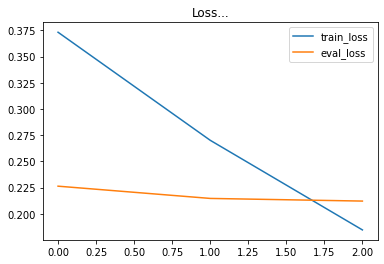
\includegraphics[width= 0.9\linewidth]{gambar/loss_concat_awal.png}
        \caption{Nilai \textit{Loss} saat Pengujian dengan Mengambil Bagian Awal Teks}
        \label{fig: loss_const_awal}
    \end{center}
\end{figure}


\subsection{Pengujian dengan Mengambil Bagian Akhir Teks}

Mirip seperti pengujian dengan mengambil bagian awal teks, terdapat ciri - ciri lain yang biasanya terdapat pada teks berita berbahasa Indonesia adalah adanya kesimpulan pada bagian akhir teks berita. Sehingga, setelah isi berita yang biasanya dibahas cukup dalam, pembaca dapat mengetahui bagaimana dan apa hubungan setiap informasi yang disajikan dengan peristiwa yang sedang dibahas dalam berita.

Dapat dilihat pada tabel \ref{tab: const_akhir}, model dengan cara memotong teks seperti ini berhasil mendapatkan tingkat akurasi sebesar 86\%. Namun, apabila melihat nilai \textit{recall} dan \textit{precision}-nya, ada indikasi bias dimana model lebih memiliki kecenderungan untuk mengeluarkan hasil hoaks bahkan pada berita valid sekalipun. Sedangkan, apabila melihat pada gambar \ref{fig: loss_const_akhir}, dapat dilihat bahwa baik nilai \textit{train loss} dan \textit{validation loss} sudah berada di titik optimal dan apabila dilakukan \textit{training} tambahan, akan membuat model \textit{overfit}.

\begin{table}
    \caption{Hasil Pengujian dengan Mengambil Akhir Teks}
    \label{tab: const_akhir}
    \centering
    \begin{tabular}{|l|l|l|}
        \hline
        \multicolumn{2}{|l|}{\textbf{Hasil Model}} & \textbf{Nilai}        \\ \hline
        \multirow{4}{*}{\textit{Confusion Matrix}} & TP             & 121  \\ \cline{2-3}
                                                   & FP             & 23   \\ \cline{2-3}
                                                   & TN             & 130  \\ \cline{2-3}
                                                   & FN             & 18   \\ \hline
        \multirow{2}{*}{\textit{Recall}}           & Hoax           & 88\% \\ \cline{2-3}
                                                   & Valid          & 84\% \\ \hline
        \multirow{2}{*}{\textit{Precision}}        & Hoax           & 85\% \\ \cline{2-3}
                                                   & Valid          & 87\% \\ \hline
        \multirow{2}{*}{\textit{F1-Score}}         & Hoax           & 86\% \\ \cline{2-3}
                                                   & Valid          & 86\% \\ \hline
        \multicolumn{2}{|l|}{\textit{Accuracy}}    & 86\%                  \\ \hline
    \end{tabular}
\end{table}

\begin{figure}[h]
    \begin{center}
        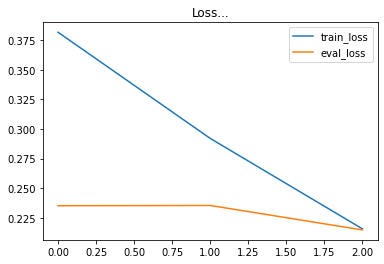
\includegraphics[width= 0.9\linewidth]{gambar/loss_concat_akhir.png}
        \caption{Nilai \textit{Loss} saat Pengujian dengan Mengambil Bagian Akhir Teks}
        \label{fig: loss_const_akhir}
    \end{center}
\end{figure}

\subsection{Pengujian dengan Mengambil Bagian Awal dan Akhir Teks}

Pengujian ini berdasarkan pada penelitian Chi Sun et al. yang menemukan bahwa dengan strategi pengambilan teks yang dibagi dua seperti ini akan dapat memberikan nilai akurasi yang lebih baik apabila dibandingkan dengan mengambil hanya di bagian awal maupun di bagian akhir saja \cite{sun2019fine}. Alasan dari penyebab lebih tingginya akurasi adalah karena dengan mengambil sebagian di awal maka sebagian dari ringkasan berita akan didapatkan, sedangkan mengambil sebagian di akhir adalah agar kesimpulan berita juga masuk ke dalam proses \textit{training}. Namun, pengujian tersebut dilakukan pada dataset teks berita berbahasa Inggris sehingga masih harus dilakukan pengujian lagi pada dataset teks berita berbahasa Indonesia.

\begin{table}[]
    \caption{Hasil Pengujian dengan Mengambil Tengah Teks}
    \label{tab: const_tengah}
    \centering
    \begin{tabular}{|l|l|l|}
        \hline
        \multicolumn{2}{|l|}{\textbf{Hasil Model}} & \textbf{Nilai}        \\ \hline
        \multirow{4}{*}{\textit{Confusion Matrix}} & TP             & 120  \\ \cline{2-3}
                                                   & FP             & 19   \\ \cline{2-3}
                                                   & TN             & 134  \\ \cline{2-3}
                                                   & FN             & 19   \\ \hline
        \multirow{2}{*}{\textit{Recall}}           & Hoax           & 88\% \\ \cline{2-3}
                                                   & Valid          & 86\% \\ \hline
        \multirow{2}{*}{\textit{Precision}}        & Hoax           & 88\% \\ \cline{2-3}
                                                   & Valid          & 86\% \\ \hline
        \multirow{2}{*}{\textit{F1-Score}}         & Hoax           & 88\% \\ \cline{2-3}
                                                   & Valid          & 86\% \\ \hline
        \multicolumn{2}{|l|}{\textit{Accuracy}}    & 87\%                  \\ \hline
    \end{tabular}
\end{table}

\begin{figure}[h]
    \begin{center}
        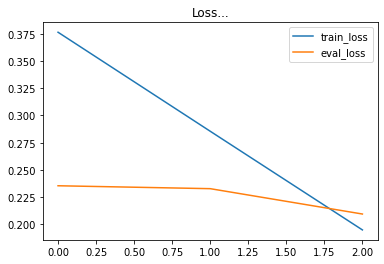
\includegraphics[width= 0.9\linewidth]{gambar/loss_concat_tengah.png}
        \caption{Nilai \textit{Loss} saat Pengujian dengan Mengambil Bagian Tengah Teks}
        \label{fig: loss_const_tengah}
    \end{center}
\end{figure}


\section{Pengujian Performa berdasarkan model BERT yang digunakan}

Terdapat banyak sekali model BERT yang sudah dibuat oleh berbagai orang di internet, ada model yang memiliki kemampuan \textit{multilanguage} sehingga bisa digunakan di berbagai bahasa sekaligus, namun kebanyakan model yang beredar adalah model yang menggunakan bahasa yang spesifik. Hal ini karena waktu \textit{pre-training} yang lebih singkat karena dataset yang lebih sedikit apabila dibandingkan model dengan kemampuan \textit{multilanguage} dan karena waktu \textit{pre-training} lebih sedikit, maka sumber daya yang digunakan juga menjadi lebih sedikit. Selain itu, dan hal ini adalah yang paling penting, hasil akurasi dari model yang hanya menggunakan 1 bahasa memiliki tingkat akurasi yang lebih tinggi apabila dibandingkan dengan model dengan banyak bahasa sekaligus. Maka dari itu, kami menguji pada beberapa model BERT sekaligus dengan rincian nama model sebagai berikut :

\begin{enumerate}[nolistsep]
    \item Model khusus bahasa Melayu, diwakili oleh : \textit{bert-base-bahasa-standard-case}
    \item Model dengan multibahasa, diwakili oleh : \textit{bert-multilingual-uncased}
    \item Model khusus bahasa Indonesia, \textit{indobert-base-p1}
    \item Model khusus bahasa Indonesia, \textit{bert-base-indonesian-522M}
    \item Model khusus bahasa Indonesia, \textit{bert-base-indonesian-1.5G}
\end{enumerate}

\begin{table}
    \centering
    \caption{Konfigurasi yang digunakan oleh model BERT yang digunakan}
    \label{tab:multi_bert_config}
    \begin{tabular}{|p{.5\linewidth}|c|l|p{.12\linewidth} |}
        \hline
        Model                          & epoch & dropout & learning rates \\ \hline
        bert-base-bahasa-standard-case & 4     & 0.2     & 2e-5           \\ \hline
        bert-base-multilingual-uncased & 4     & 0.2     & 2e-5           \\ \hline
        indobert-base-p1               & 3     & 0.1     & 2e-5           \\ \hline
        bert-base-indonesian-522M      & 3     & 0.1     & 2e-5           \\ \hline
        bert-base-indonesian-1.5G      & 3     & 0.2     & 2e-5           \\ \hline
    \end{tabular}
\end{table}

Untuk melakukan \textit{training}, sebelumnya kami mengatur konfigurasi yang akan digunakan oleh model BERT yang sudah disiapkan. Terdapat beberapa perbedaan pada konfigurasi seperti jumlah \textit{epoch} dan jumlah \textit{dropout}. Hal ini agar membuat model dapat memiliki konfigurasi yang lebih optimal dan tidak mengalami \textit{overfit} maupun \textit{underfit}.

\subsection{Pengujian pada model khusus bahasa Melayu}

Model yang diberi nama \textit{bert-base-bahasa-standard-case} adalah model yang di-\textit{pretrained} menggunakan bahasa Melayu saja dengan mengambil berbagai sumber dataset seperti media sosial, Wikipedia, sampai Wattpad \cite{Malaya}. Model ini dilatih oleh huzeinzol05 dan menurut pembuat model, model ini seharusnya dapat digunakan baik untuk tugas - tugas berbahasa Melayu maupun tugas - tugas berbahasa Indonesia dikarenakan kesamaan pada tata bahasa dan arti suatu kata. Dalam buku ini model ini disebutkan dengan \textit{bert-bahasa}

\begin{figure}[h]
    \begin{center}
        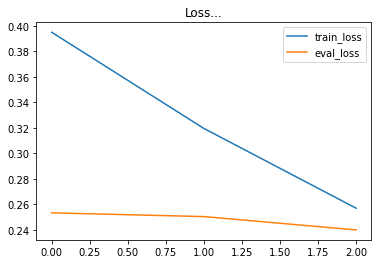
\includegraphics[width= 0.9\linewidth]{gambar/loss_bert_bahasa.png}
        \caption{Nilai \textit{Loss} saat Pengujian dengan model \textit{bert-bahasa}}
        \label{fig: loss_bert_bahasa}
    \end{center}
\end{figure}

\begin{table}
    \caption{Hasil Pengujian dengan model \textit{bert-bahasa}}
    \label{tab: loss_bahasa}
    \centering
    \begin{tabular}{|l|l|l|}
        \hline
        \multicolumn{2}{|l|}{\textbf{Hasil Model}} & \textbf{Nilai}        \\ \hline
        \multirow{4}{*}{\textit{Confusion Matrix}} & TP             & 124  \\ \cline{2-3}
                                                   & FP             & 28   \\ \cline{2-3}
                                                   & TN             & 125  \\ \cline{2-3}
                                                   & FN             & 15   \\ \hline
        \multirow{2}{*}{\textit{Recall}}           & Hoax           & 89\% \\ \cline{2-3}
                                                   & Valid          & 82\% \\ \hline
        \multirow{2}{*}{\textit{Precision}}        & Hoax           & 82\% \\ \cline{2-3}
                                                   & Valid          & 89\% \\ \hline
        \multirow{2}{*}{\textit{F1-Score}}         & Hoax           & 85\% \\ \cline{2-3}
                                                   & Valid          & 85\% \\ \hline
        \multicolumn{2}{|l|}{\textit{Accuracy}}    & 85\%                  \\ \hline
    \end{tabular}
\end{table}

Pada gambar \ref{fig: loss_bert_bahasa} terlihat bahwa model memiliki nilai \textit{validation loss} dan \textit{training loss} yang cukup bagus. Namun, apabila diuji dengan menambahkan epoch, hasil pengujian tersebut menghasilkan model yang \textit{overfitting} sehingga tidak kami gunakan sebagai nilai pembanding. Berdasarkan tabel \ref{tab: loss_bahasa}, terlihat bahwa \textit{recall} lebih tinggi dibanding \textit{precision} saat mendeteksi berita hoaks, sehingga dapat disimpulkan bahwa model mengalami kesulitan saat digunakan untuk mendeteksi berita yang valid.

\subsection{Pengujian pada model dengan kemampuan multibahasa}

Model BERT yang digunakan pada pengujian ini adalah model dasar yang dibuat langsung oleh tim di Google. Selain itu, model ini jugalah yang merupakan hasil dari penelitian yang sudah dibuat oleh devlin et al. dalam penelitian awal mengenai BERT. Model ini dilatih pada seluruh bahasa yang ada pada Wikipedia sehingga untuk saat ini, model tersebut dapat mendukung sebanyak 104 bahasa sekaligus termasuk didalamnya adalah bahasa Indonesia. Oleh tim dari Google, model ini diberi nama \textit{bert-base-multilingual-uncased} dan dalam buku ini disingkat sebagai \textit{bert-base}.

\begin{figure}[h]
    \begin{center}
        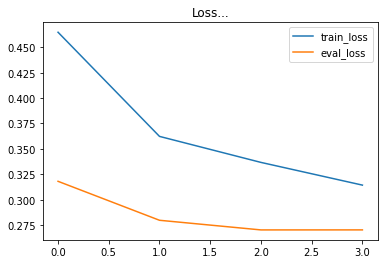
\includegraphics[width= 0.9\linewidth]{gambar/loss_bert_multilingual.png}
        \caption{Nilai \textit{Loss} saat Pengujian dengan model \textit{bert-base}}
        \label{fig: loss_bert_multilingual}
    \end{center}
\end{figure}

\begin{table}[h]
    \caption{Hasil Pengujian dengan model \textit{bert-base}}
    \label{tab: loss_multilingual}
    \centering
    \begin{tabular}{|l|l|l|}
        \hline
        \multicolumn{2}{|l|}{\textbf{Hasil Model}} & \textbf{Nilai}        \\ \hline
        \multirow{4}{*}{\textit{Confusion Matrix}} & TP             & 135  \\ \cline{2-3}
                                                   & FP             & 38   \\ \cline{2-3}
                                                   & TN             & 115  \\ \cline{2-3}
                                                   & FN             & 4    \\ \hline
        \multirow{2}{*}{\textit{Recall}}           & Hoax           & 97\% \\ \cline{2-3}
                                                   & Valid          & 78\% \\ \hline
        \multirow{2}{*}{\textit{Precision}}        & Hoax           & 75\% \\ \cline{2-3}
                                                   & Valid          & 97\% \\ \hline
        \multirow{2}{*}{\textit{F1-Score}}         & Hoax           & 85\% \\ \cline{2-3}
                                                   & Valid          & 87\% \\ \hline
        \multicolumn{2}{|l|}{\textit{Accuracy}}    & 86\%                  \\ \hline
    \end{tabular}
\end{table}

Mirip seperti pada model \textit{bert-bahasa}, model \textit{bert-base} ini adalah model dengan grafik yang cukup bagus, terlihat pada gambar \ref{fig: loss_bert_multilingual}, nilai dari \textit{training loss} memilki \textit{trend} yang kurang lebih sama apabila dibandingkan dengan nilai \textit{validation loss}. Namun, apabila melihat dari tabel \ref{tab: loss_multilingual} nilai dari \textit{recall} dan \textit{precision}-nya menunjukkan model kesulitan dalam mendeteksi berita valid.

\subsection{Pengujian pada model \textit{indobert-base-p1}}

Model BERT ini adalah salah satu dari 3 model khusus berbahasa Indonesia yang diuji dalam penelitian ini. Dibuat oleh tim indobenchmarksebagai bagian dari penelitian untuk uji \textit{benchmarking} pada \textit{Natural Language Understanding} (NLU) berbahasa Indonesia. Diantara model - model BERT khusus bahasa Indonesia yang lain, model ini adalah model yang dilatih pada dataset terbanyak, yaitu sebesar 23 GB lebih data yang berasal dari banyak sumber seperti Wikipedia, sosial media, OpenSubtitle, dan banyak lagi \cite{koto2020indolem}.

\begin{figure}[h]
    \begin{center}
        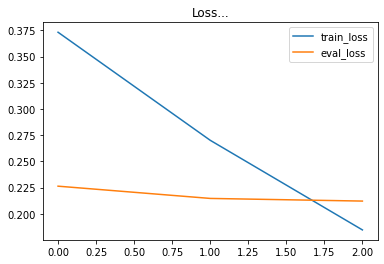
\includegraphics[width= 0.9\linewidth]{gambar/loss_concat_awal.png}
        \caption{Nilai \textit{Loss} saat Pengujian dengan model \textit{indobert}}
        \label{fig: loss_bert_indobert}
    \end{center}
\end{figure}

\begin{table}[h]
    \caption{Hasil Pengujian dengan model \textit{indobert}}
    \label{tab: loss_indobert}
    \centering
    \begin{tabular}{|l|l|l|}
        \hline
        \multicolumn{2}{|l|}{\textbf{Hasil Model}} & \textbf{Nilai}        \\ \hline
        \multirow{4}{*}{\textit{Confusion Matrix}} & TP             & 122  \\ \cline{2-3}
                                                   & FP             & 16   \\ \cline{2-3}
                                                   & TN             & 137  \\ \cline{2-3}
                                                   & FN             & 17   \\ \hline
        \multirow{2}{*}{\textit{Recall}}           & Hoax           & 89\% \\ \cline{2-3}
                                                   & Valid          & 88\% \\ \hline
        \multirow{2}{*}{\textit{Precision}}        & Hoax           & 90\% \\ \cline{2-3}
                                                   & Valid          & 88\% \\ \hline
        \multirow{2}{*}{\textit{F1-Score}}         & Hoax           & 89\% \\ \cline{2-3}
                                                   & Valid          & 88\% \\ \hline
        \multicolumn{2}{|l|}{\textit{Accuracy}}    & 89\%                  \\ \hline
    \end{tabular}
\end{table}

Sebagai model yang dilatih pada dataset khusus berbahasa Indonesia yang paling banyak, model ini memiliki tingkat akurasi yang paling tinggi apabila dibanding model - model yang lain. Gambar \ref{fig: loss_bert_indobert} menunjukkan grafik \textit{loss} dari model ini, terlihat pada grafik tersebut, nilai \textit{validation loss} nya sudah lebih tinggi dari \textit{training loss}-nya sehingga model sudah sedikit \textit{overfit}.


